
\begin{figure*}[t]
    \centering
    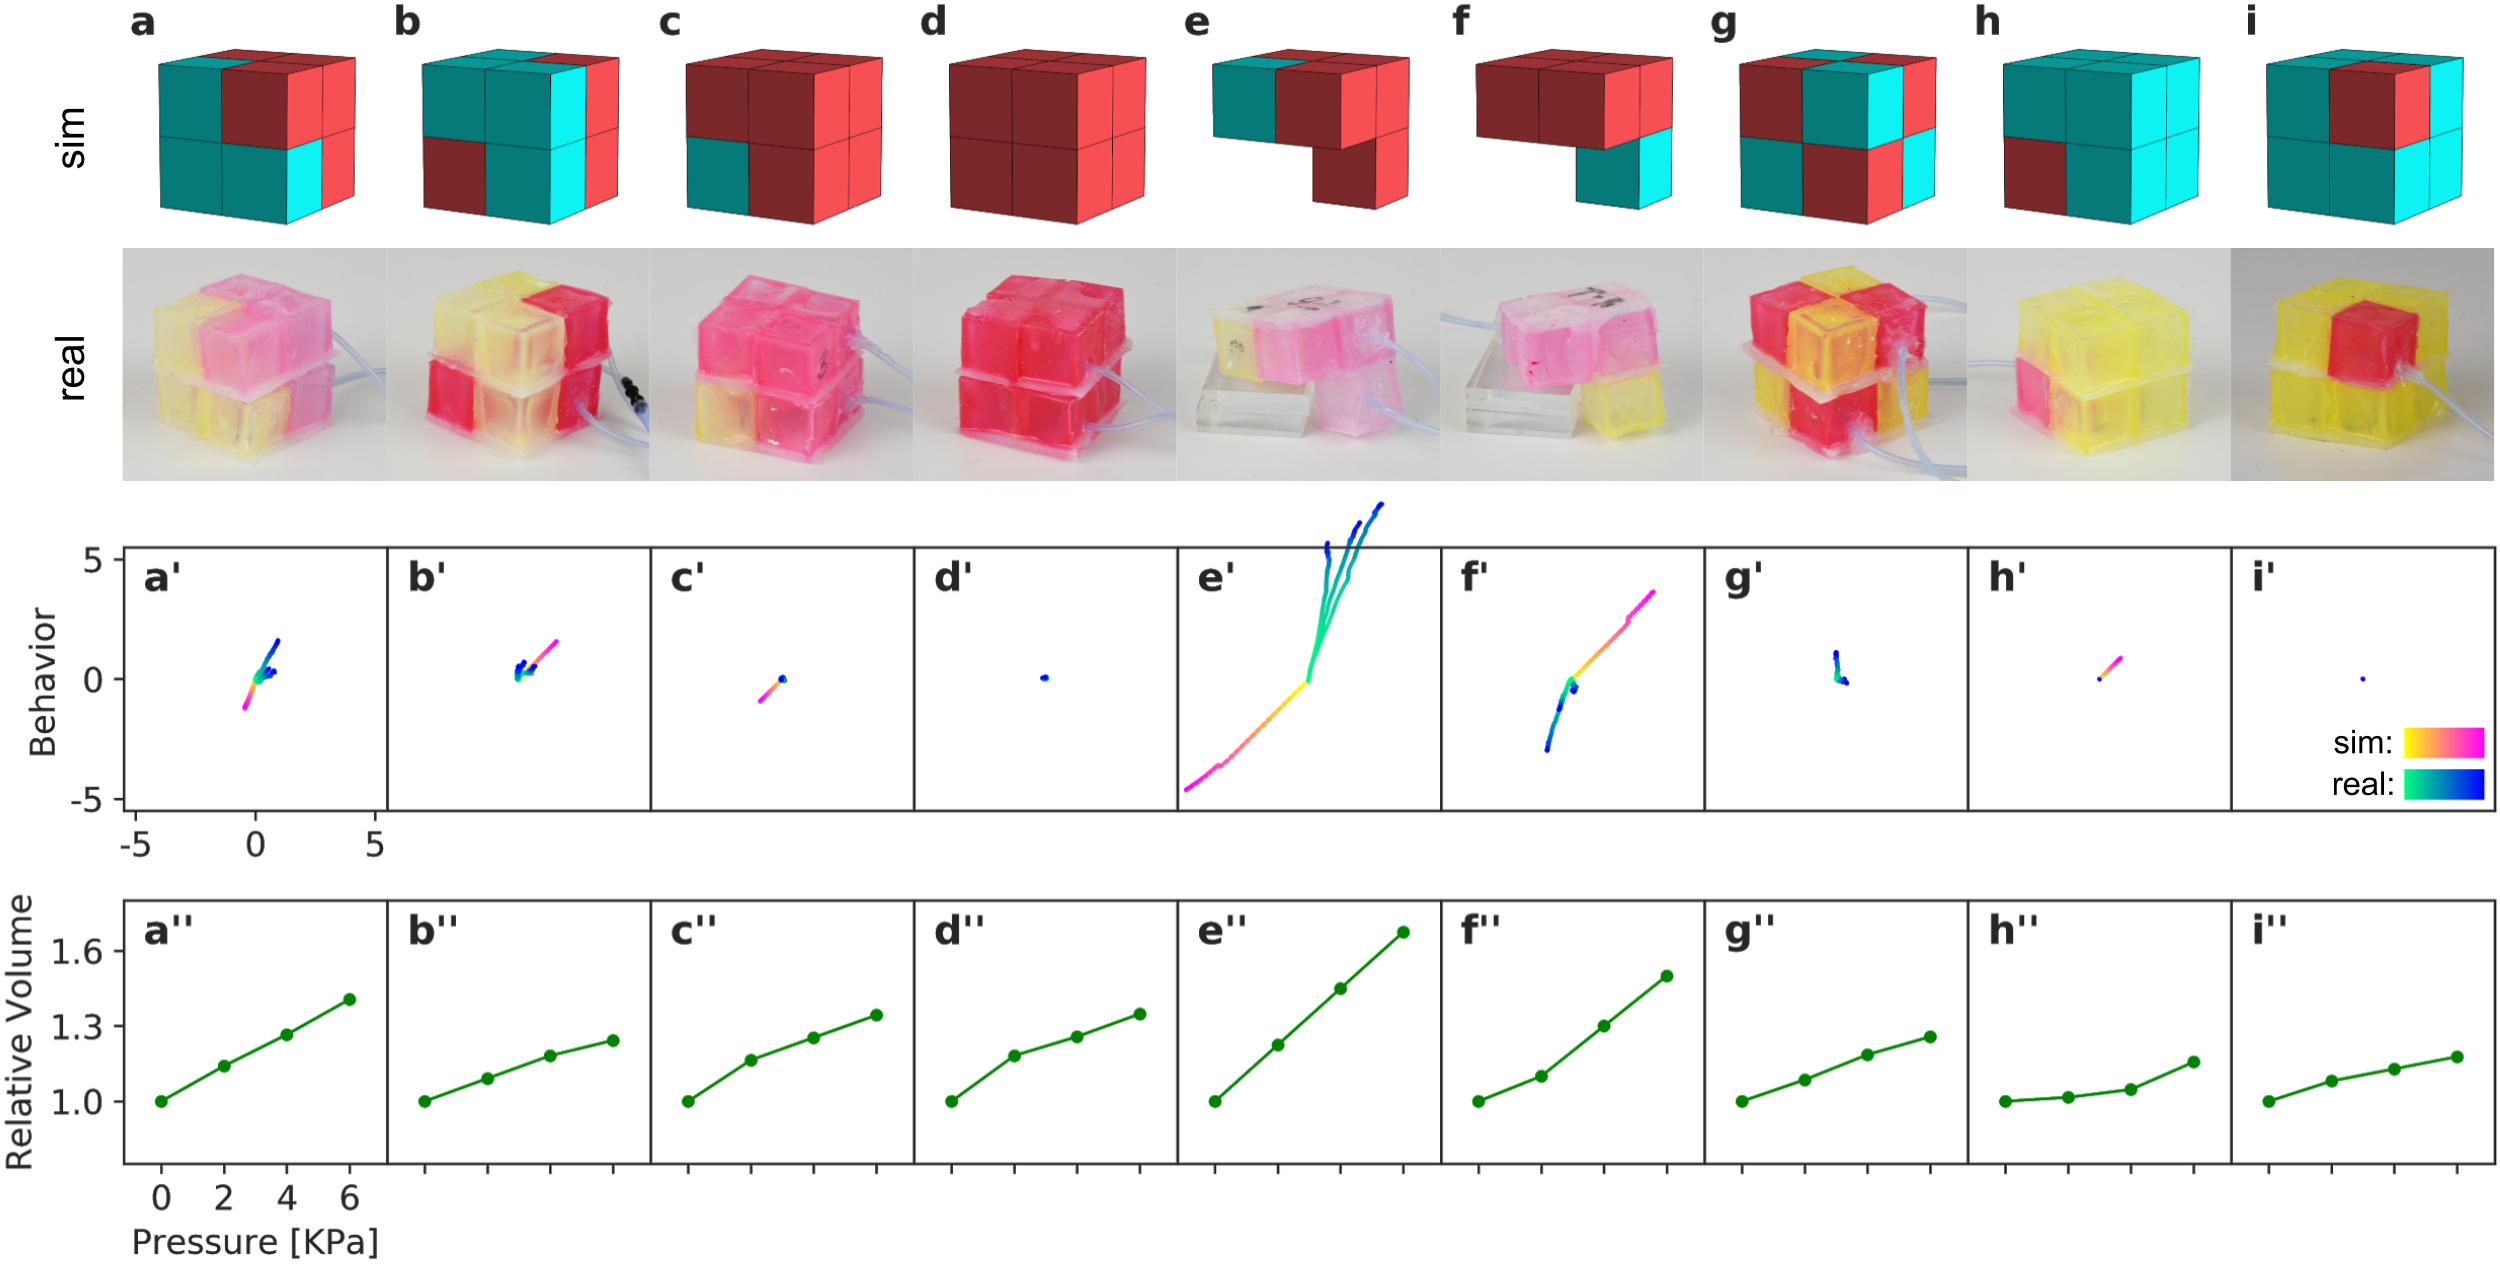
\includegraphics[width=\linewidth]{Chapter02/fig/YaleTraces2.png}
    % \vspace{-1.75em}
    \caption{\textbf{Measuring transferal from simulation to reality}.
    Nine designs (\textbf{a-i}) were evaluated three times each in reality (green-to-blue gradient colored curves in \textbf{a\textquotesingle-i\textquotesingle}).
    The behavioral trajectories start at the origin (green) and end at the robot's final XY destination (blue) (in centimeters).
    The simulated movement tracks (yellow-to-pink curves) are superimposed on top of the real ones.
    The relative volume (normalized by rest volume) was also recorded for each design at four points during actuation under water (\textbf{a\textquotesingle\textquotesingle-i\textquotesingle\textquotesingle}).
    % The two designs that displaced farthest in the plane (e and f) also achieved the largest volumetric expansion.
    The simulated and real behavior of designs e and f can be observed here:
    \href{https://youtu.be/UqjvmkYa9u4}{\color{blue}\tt\textbf{youtu.be/UqjvmkYa9u4}}.
    }
    \label{fig:transfer}
    % \vspace{-1.25em}
\end{figure*}
